\chapter[扩展定律与效率]{扩展定律与高效大语言模型}\label{chap:scaling}

\begin{learningbox}
本章将介绍语言模型的性能如何随着数据量与训练投入的增加而变化。
具体而言，学完本章后，你将能够：
\begin{itemize}[leftmargin=*, nosep]
    \item 解释模型性能如何通过{\em 扩展定律（scaling law）}与计算量、数据量及模型规模相关联，并预测在其他因素不变时增加某一因素会产生什么影响。
    \item 说明哪些技术可以用于开发{\em 更小的语言模型}，并从计算需求与性能两方面分析使用较小模型的权衡。
    \item 区分{\em 推理阶段计算量（inference-time compute）}与训练阶段计算量。
    \item 思考\emph{可持续语言模型}，以及大规模部署对环境和隐私的影响。
\end{itemize}
\end{learningbox}

\section{扩展定律：计算量、数据量与参数量}
\label{sec:scaling-laws}
大语言模型的训练涉及三个主要因素：\begin{enumerate*}[label=(\arabic*)]
    \item 计算量；
    \item 数据集规模；
    \item 模型规模。
\end{enumerate*}
研究表明，这三个因素与模型的最终性能有关；这里用模型在留出测试集上的损失（$L$）来衡量性能。人们发现，这种关系既平滑又可预测。它呈现为一种\emph{幂律（power law）}：增加上述任意一种资源，损失就会按照该资源的某个负次幂成比例地下降。例如，将模型规模增加一倍，可能使损失变为原来的 $2^{-\alpha}$，其中 $\alpha$ 是某个正指数。由于这种变化可以预测，我们能够在投入昂贵的训练之前，\emph{预先}估计模型会改善多少，例如将训练数据集规模增加一倍所带来的改善。

我们将这三个量（$C$、$D$、$N$）定义如下：
\begin{itemize}
    \item 计算量（$C$）：整个训练过程中执行的算术运算总量，以浮点运算次数（floating point operations，FLOPs）衡量。注意，这里计算的是运算总次数，而不是每秒运算次数。一个广泛使用的近似关系将它与另外两个量联系起来：$C \approx 6ND$。这是因为，处理一个词元时，前向传播和反向传播对 $N$ 个参数中的每一个大约分别进行两次和四次运算，合计约六次。
    \item 数据集规模（$D$）：模型训练所使用的词元总数。注意，词元是由词元化器定义的子词单元，因此，同一语料库在不同词元化器下会对应不同的 $D$ 值。$D$ 统计的是训练过程中实际使用的词元数量。当数据在多个训练轮次中重复使用时，重复出现的词元仍会计入 $D$，但与新数据相比，其收益可能递减。
    \item 模型规模（$N$）：模型架构中可训练参数（权重）的数量。这个数通常只包括随模型深度扩展而增加的参数，因此不包括嵌入矩阵。
\end{itemize}
训练大模型需要付出相当高的成本，通常达到数千万美元，计算时间则可能长达数月。扩展定律让我们能够预测模型能否得到良好的训练。

\begin{figure}[t]
    \centering
    % 原始数据图保持不变；只覆盖图外的英文轴题与单位说明。
\begin{tikzpicture}
\node[anchor=south west,inner sep=0] (plot) at (0,0) {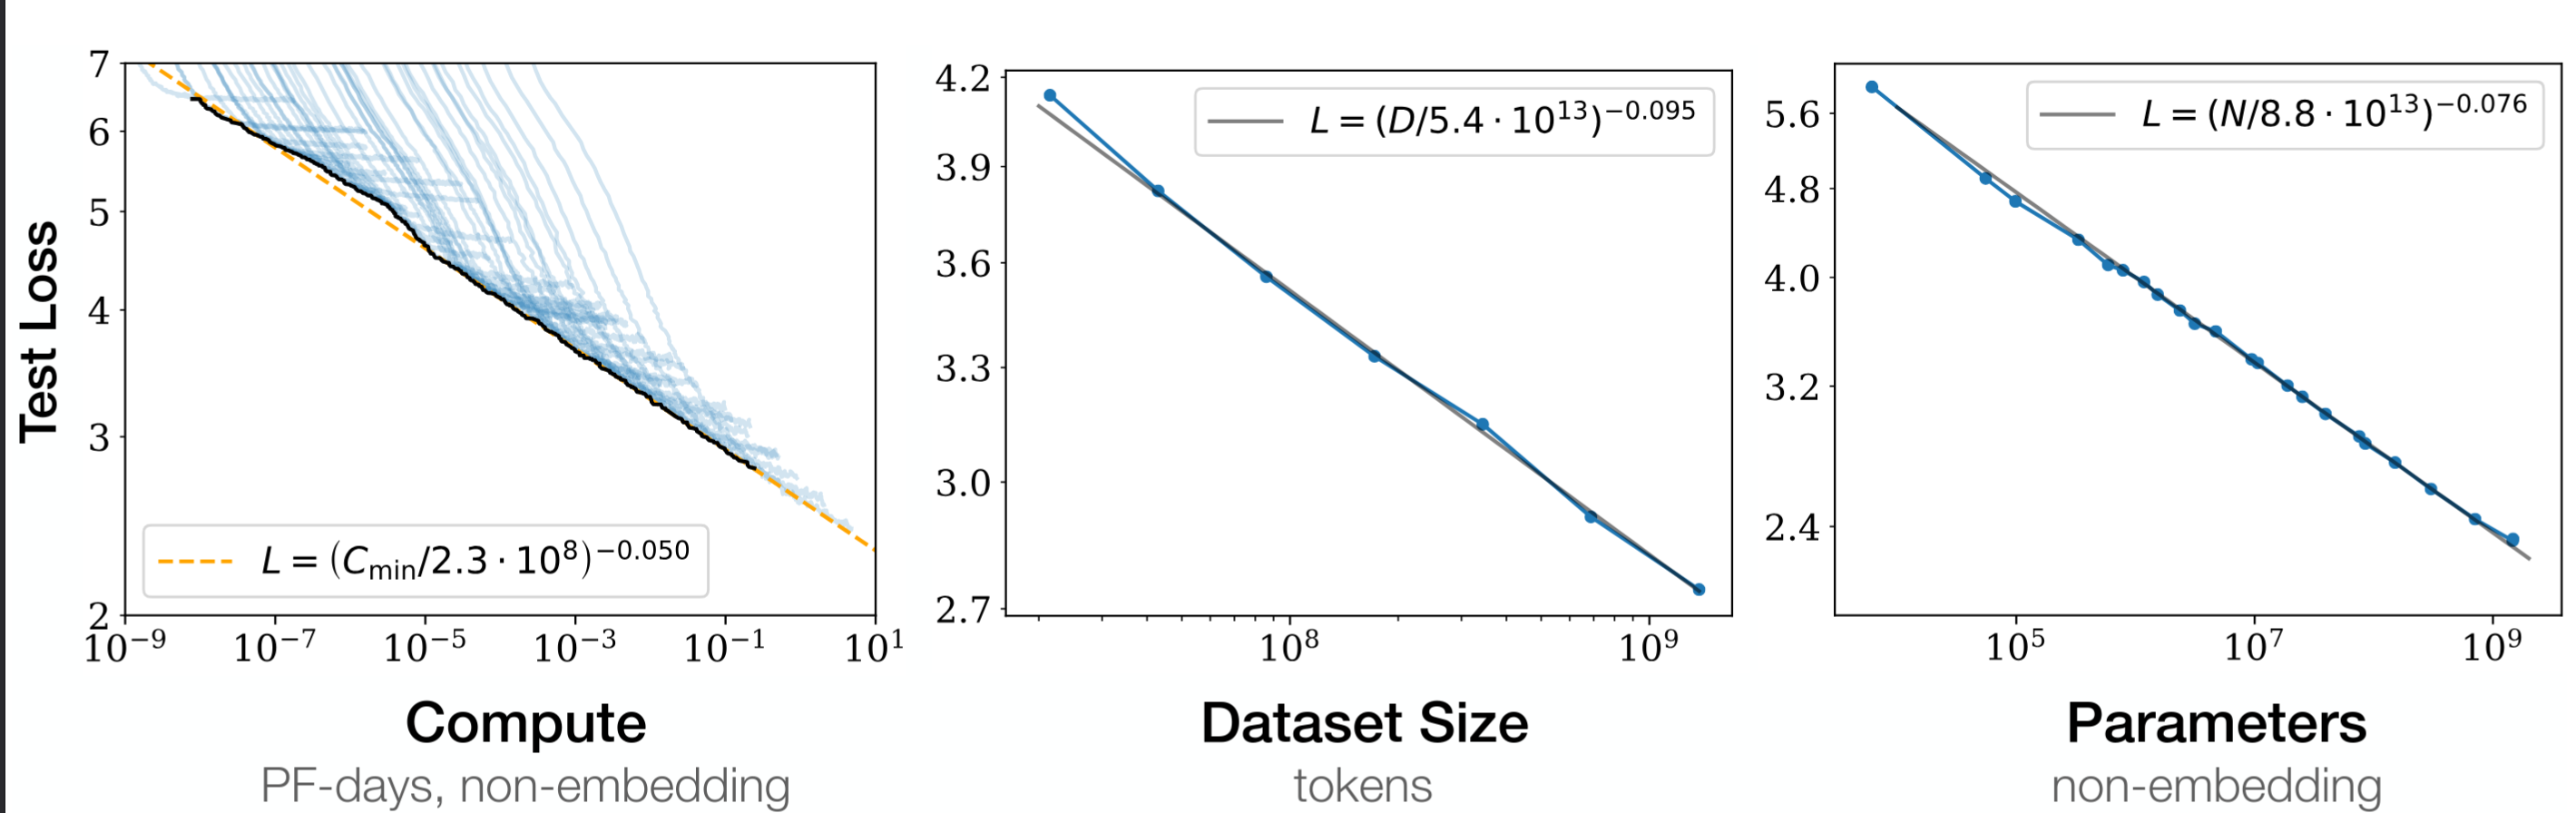
\includegraphics[width=.9\linewidth]{part1/visuals/scaling.png}};
\begin{scope}[x={(plot.south east)},y={(plot.north west)},every node/.style={font=\scriptsize,inner sep=0pt}]
\fill[white] (-.002,-.001) rectangle (.008,1.001);
\fill[white] (0,.20) rectangle (.035,.85);
\node[rotate=90] at (.015,.56) {测试损失};
\fill[white] (.045,0) rectangle (.995,.145);
\node at (.205,.108) {计算量};
\node at (.205,.025) {PF-days，不含嵌入参数};
\node at (.530,.108) {数据集规模};
\node at (.530,.025) {词元数};
\node at (.855,.108) {参数量};
\node at (.855,.025) {不含嵌入参数};
\end{scope}
\end{tikzpicture}

    \caption{语言建模目标上的损失是训练计算量、数据集规模和模型规模的函数 \citep{kaplan2020scalinglawsneurallanguage}。}
    \label{fig:scaling-law}
\end{figure}

\subsection{Kaplan 扩展定律}
通过对实验测试数据拟合函数，可以得到不同的扩展定律经验结果。例如，图~\ref{fig:scaling-law}~中的每一个点，都对应一个在固定数据集上训练得到的模型，各模型采用相似的实验设置，只改变三个主要变量 $C,D,N$。2020 年初，\citet{kaplan2020scalinglawsneurallanguage} 发现了模型性能与 $C,D,N$ 的关系。
他们根据实验观测估计，损失分别遵循与这三个主要变量有关的独立幂律：$L(N) \propto N^{-\alpha_N}$ 和 $L(D) \propto D^{-\alpha_D}$，其中 $\alpha_N \approx 0.076$，$\alpha_D \approx 0.095$。

这些单独的幂律可以合并为一个能够求最优解的方程，如式~\ref{eq:joint-power}~所示。研究者假定，这种关系具有普遍性，可以很好地描述“其他生成式建模任务”的损失变化 \citep[p. 5]{kaplan2020scalinglawsneurallanguage}。作者进一步表明，如果除了计算预算以外没有其他约束，那么他们的推导就能给出最优模型规模 $N$ 和理想数据集规模 $D$，后者由最优步数（$S$）与批量大小（$B$）确定。

\begin{equation}
\label{eq:joint-power}
L(N, D) = \Big[ \Big(\frac{N_c}{N}\Big)^{\frac{\alpha_N}{\alpha_D}} + \frac{D_c}{D} \Big]^{\alpha_D}
\end{equation}

具体而言，他们得出的结论是：随着计算预算 $C$ 增加，模型规模 $N$ 的增长速度应当快于数据规模 $D$（$N \propto C^{0.73}$，$D \propto C^{0.27}$\footnote{$B\propto C^{0.24},\,S\propto C^{0.03},\, D=B\cdot S \propto C^{0.27}$}）。这一结论推动了 GPT-3 等大模型的开发。负指数体现了收益递减：模型规模或数据集规模每增加一倍，损失只会下降几个百分点。

乍看之下，这个建议似乎与指数本身相矛盾：由于 $\alpha_D > \alpha_N$，在计算量相对增幅相同的情况下，扩展数据比扩展参数能\emph{更快}地降低损失。原因在于，约束条件是计算量，而不是资源本身：由于 $C \approx 6ND$，增加 $D$ 与增加 $N$ 一样都要消耗计算量。这意味着，$N$ 越来越可能成为瓶颈。因此，将 $D$ 的计算成本考虑在内之后，把额外计算量分配给 $N$，比将其分配给 $D$ 能获得更好的回报。这也就意味着，最优分配偏向更大的模型。

\paragraph{样本效率}
\citet{kaplan2020scalinglawsneurallanguage} 还观察到，更大的模型具有更高的\emph{样本效率（sample efficiency）}。在训练词元数量固定时，更大的模型能达到更低的损失；而要达到给定的目标损失，与较小模型相比，它所需的词元和优化步数也更少。图~\ref{fig:sample-efficiency-tokens}~展示了这一效应。

\begin{figure}[t]
    \centering
    % 原图的点、曲线、刻度与图例数值不变，只叠加中文文字。
\begin{tikzpicture}
\node[anchor=south west,inner sep=0] (plot) at (0,0) {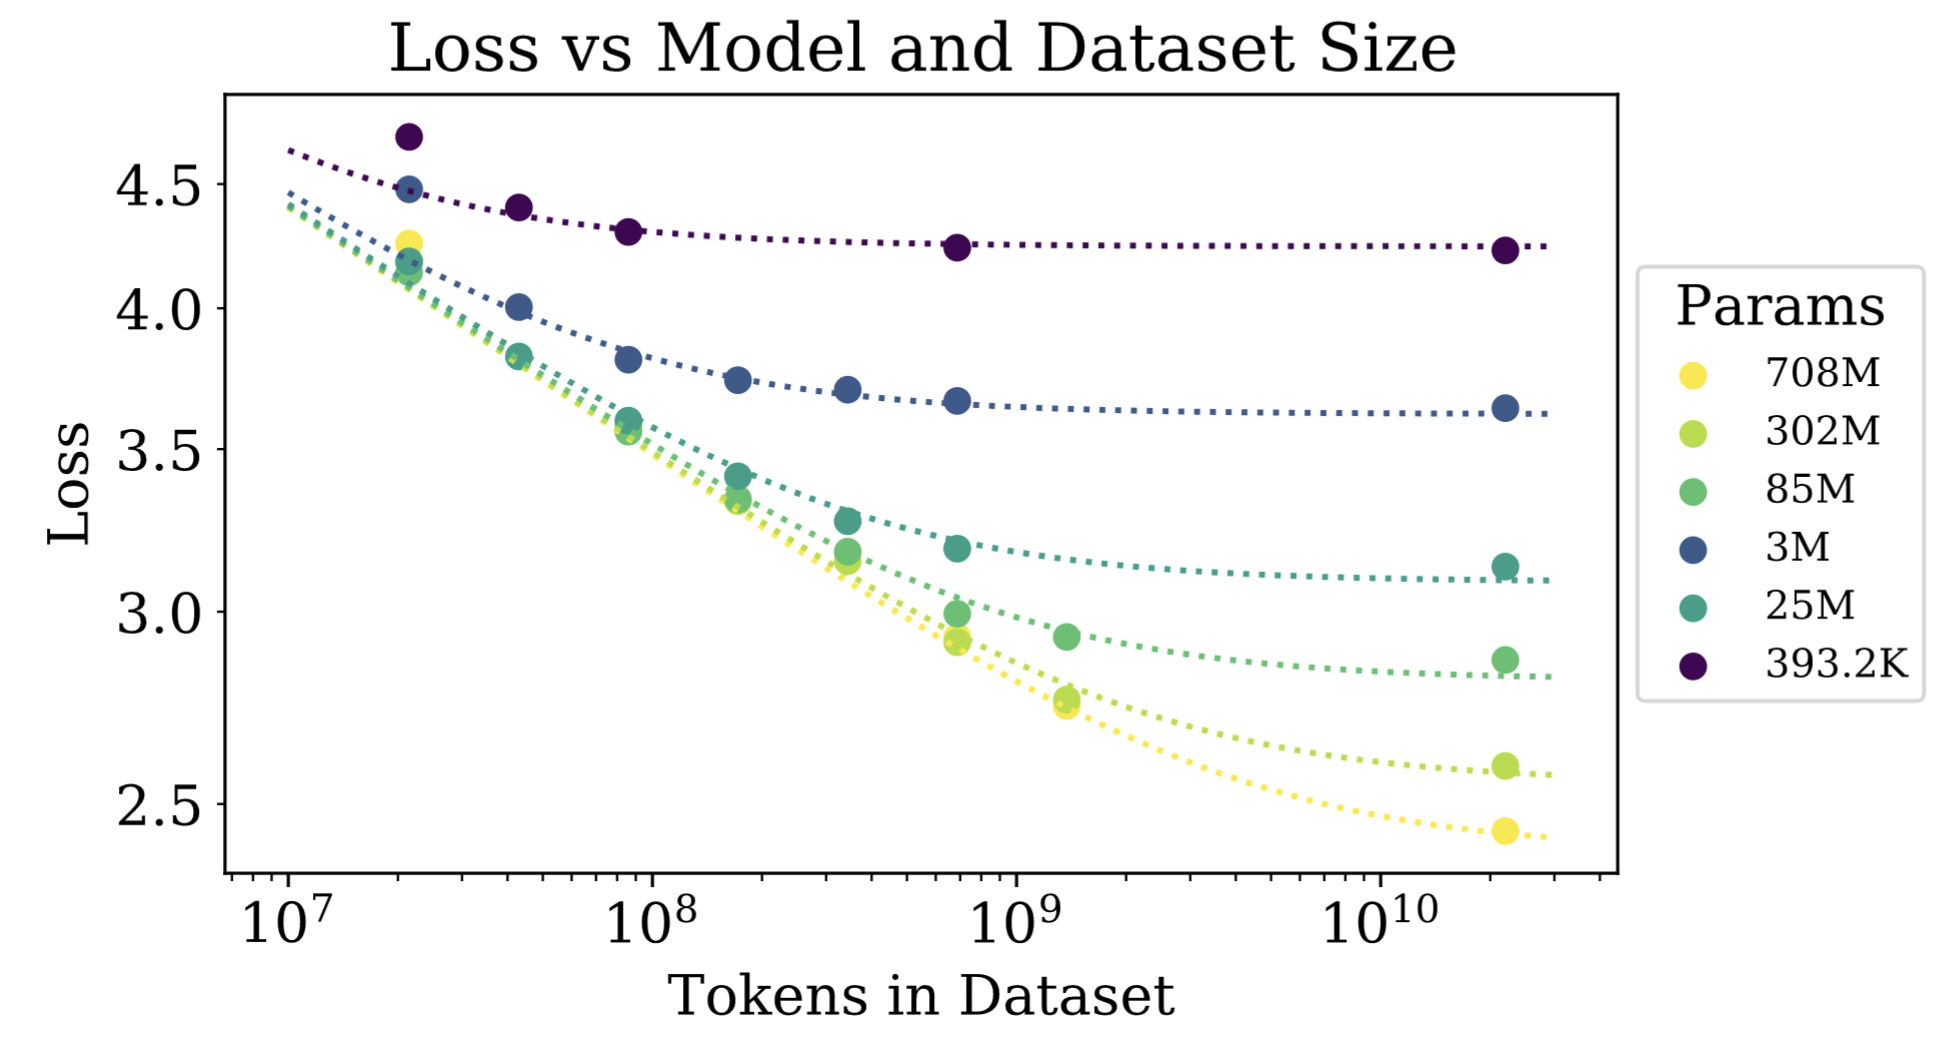
\includegraphics[width=.7\linewidth]{part1/visuals/sample_efficiency_tokens.png}};
\begin{scope}[x={(plot.south east)},y={(plot.north west)},every node/.style={font=\scriptsize,inner sep=0pt}]
\fill[white] (.15,.915) rectangle (.85,1);
\node[font=\small] at (.5,.965) {损失与模型规模、数据集规模的关系};
\fill[white] (0,.40) rectangle (.05,.75);
\node[rotate=90] at (.026,.55) {损失};
\fill[white] (.30,0) rectangle (.77,.092);
\node at (.53,.035) {数据集中的词元数};
\fill[white] (.845,.685) rectangle (.99,.755);
\node at (.918,.72) {参数量};
\end{scope}
\end{tikzpicture}

    \caption{更大的模型用更少的训练词元就能达到给定损失，体现出更高的样本效率 \citep{kaplan2020scalinglawsneurallanguage}。}
    \label{fig:sample-efficiency-tokens}
\end{figure}

\subsection{Chinchilla 扩展定律}
2022 年，\citet{10.5555/3600270.3602446} 使用一个名为 Chinchilla 的模型重新评估了这些发现，并意外地发现，当时大多数大模型都严重训练不足。这一差异可以追溯到 \citet{kaplan2020scalinglawsneurallanguage} 的研究方法：他们的最优分配，是从许多模型\emph{早期}、尚未收敛的训练动态中外推得到的，而不是基于训练至收敛的完整过程。这使他们的结论系统性地偏向规模更大、训练步数更少的模型。

Chinchilla 研究的核心发现是：计算预算每增加一倍，模型规模 $N$ 和训练词元数 $D$ 都应当以大致相等的比例增加（$N \propto C^{0.5}$，$D \propto C^{0.5}$）。他们给出的经验法则建议，模型中的每一个可训练参数应当对应约 20 个训练词元，才能实现计算最优。此后，这一结果已被复现 \citep{besiroglu2024chinchilla}，并且被证明对于较大的扰动也具有稳健性 \citep{schaeffer2025evaluating}。

在他们的扩展定律中，损失被建模为参数量 $N$ 和已用于训练的词元数 $D$ 的函数，形式如下：
\begin{equation}
    L(N,D) = E + \frac{A}{N^{\alpha}} + \frac{B}{D^{\beta}}
\end{equation}

第一项 $E$ 表示不可约损失，对应于自然文本的熵。第二项 $\frac{A}{N^{\alpha}}$ 表示模型参数量 $N$ 有限所造成的次优性，最后一项 $\frac{B}{D^{\beta}}$ 则表示训练词元数 $D$ 有限所造成的次优性。虽然这里的 $\alpha$ 和 $\beta$ 与 Kaplan 的 $\alpha_N$ 和 $\alpha_D$ 起着相同的作用，即控制损失如何随模型规模和数据量增加而下降，但它们采用了不同的参数化方式：这些指数是在上述两项形式中联合拟合得到的，因此取值也不同。在 400 多个模型上拟合 Chinchilla 扩展函数后，得到了以下参数估计：
\begin{equation}
    E \approx 1.69, \quad A \approx 406.4, \quad B \approx 410.7, \quad \alpha \approx 0.34, \quad \beta \approx 0.28
\end{equation}

在计算预算 $C$ 固定的约束下优化这个损失函数（回顾 $C \approx 6ND$），就可以推导出任意预算 $C$ 对应的计算最优模型规模 $N_{opt}$ 和数据规模 $D_{opt}$：
\begin{equation}
    N_{opt}(C) = G \left( \frac{C}{6} \right)^a, \quad D_{opt}(C) = \frac{1}{G} \left( \frac{C}{6} \right)^b
\end{equation}
其中，$G=\big(\frac{\alpha A}{\beta B}\big)^{\frac{1}{\alpha + \beta}}$ 是常数，$a = \frac{\beta}{\alpha + \beta} \approx 0.45$，$b = \frac{\alpha}{\alpha + \beta} \approx 0.55$。

注意，$a$ 与 $b$ 并不独立：按照定义，$a+b=1$。这一点直接来自 $C \approx 6ND$，因为取对数后可得 $\log C = \log 6 + \log N + \log D$。写成 $N_{opt} \propto C^a$ 和 $D_{opt} \propto C^b$ 后，上式变为 $\log C = \text{const} + a \log C + b \log C$；只有当 $a+b=1$ 时，它才可能对所有 $C$ 成立。同样的约束也适用于 Kaplan 的指数（$0.73 + 0.27 = 1$）。Chinchilla 的不同之处在于，预算\emph{如何}在 $N$ 和 $D$ 之间分配。

这一法则近似为\emph{线性关系}，因为 $N_{opt}$ 和 $D_{opt}$ 随计算预算 $C$ 增长的速率几乎相同：它们的指数 $a \approx 0.45$ 与 $b \approx 0.55$ 很接近，因此，在计算量跨越多个数量级时，比值 $D_{opt}/N_{opt}$ 仍然接近约 $20$ 这一常数。
对这个数值，最合适的理解是：它是以真实的计算最优训练实验为依据作出的经验校准，而不是能从拟合系数中直接、精确推得的数字。Chinchilla 模型本身有 700 亿参数，使用 1.4 万亿词元训练，恰好满足 $D/N = 20$。表~\ref{tab:token-param}~展示了几个知名模型相对于这一法则的位置。低于这一比值的模型属于\emph{训练不足（undertrained）}，即对于其词元预算而言，模型过大；远高于这一比值的模型则是有意\emph{超额训练（overtrained）}，目的是得到推理阶段运行成本较低的小模型。GPT-3 和 Gopher 等早期旗舰模型远低于这一比值（$D/N \approx 1$--$2$）：它们的规模很大，但训练所用词元相对过少。
需要强调的是，$D \approx 20N$ 只在训练预算固定、目标是最小化\emph{训练}损失时才是最优的。如果模型日后要处理大量推理请求，人们往往会有意进行\emph{超额训练}，让每个参数对应远多于 $20$ 个训练词元，以额外训练成本换取一个规模更小、推理阶段运行更便宜的模型。例如，LLaMA-3 8B 的每个参数大约对应 $1900$ 个训练词元。选择这种有意为之的极度超额训练，是为了让小模型仍能达到较低损失，同时降低推理运行成本。

\begin{table}
    \centering
    \begin{tabular}{lrrrl}
        \toprule
        模型 & $N$ & $D$ & $D/N$ & 训练状态 \\
        \midrule
        Gopher \citep{rae2021scaling}            & 280B & 300B & $\approx 1$    & 训练不足 \\
        GPT-3 \citep{brown2020language}          & 175B & 300B & $\approx 1.7$  & 训练不足 \\
        Chinchilla \citep{10.5555/3600270.3602446} & 70B  & 1.4T & $20$           & 计算最优 \\
        LLaMA-1 7B \citep{touvron2023llama1}     & 7B   & 1.0T & $\approx 143$  & 超额训练 \\
        LLaMA-2 7B \citep{touvron2023llama}      & 7B   & 2.0T & $\approx 286$  & 超额训练 \\
        LLaMA-3 8B \citep{grattafiori2024llama3herdmodels} & 8B   & 15T  & $\approx 1875$ & 超额训练 \\
        \bottomrule
    \end{tabular}
    \caption{几个知名模型的词元数与参数量之比，以及它们与 Chinchilla 经验法则 $D \approx 20N$ 的关系。}
    \label{tab:token-param}
\end{table}

到目前为止，图景相当清晰：随着计算量、数据量和参数量增加，测试损失平滑、单调且可预测地下降。然而，实践中有多种因素会影响结果。下面讨论四种现象，它们分别探查这幅图景的不同边界：
\begin{enumerate*}[label=(\arabic*)]
    \item 计算最优曲线；
    \item 涌现能力；
    \item 逆向扩展；
    \item 顿悟。
\end{enumerate*}

\subsection{计算最优曲线}
计算机硬件与能源都是有限资源。一个实际问题是：如何在模型规模 $N$ 与数据集规模 $D$ 之间分配固定的计算预算 $C$，以获得尽可能好的模型？扩展定律通过\emph{计算最优前沿（compute-optimal frontier）}来回答这个问题，即找出使损失最小的 $C$ 分配方案。

通过图~\ref{fig:isoflop}~所示的\emph{等浮点运算量（IsoFLOP）}方法，可以从实验中确定这一前沿 \citep{10.5555/3600270.3602446}。对于不同规模的模型，我们选择相应的训练词元数，使最终的 FLOPs 保持不变。学习率采用余弦退火调度，余弦周期的长度设置为与目标 FLOP 数相匹配。我们会发现，损失曲线存在清晰的谷底，这意味着对于给定的 FLOP 预算，存在一个最优训练模型规模（左图）。利用这些谷底的位置，我们可以预测更大模型的最优规模与词元数（中图和右图）。绿色表示使用 Gopher 的计算预算训练最优模型时，所估计的参数量与词元数。在固定 FLOP 预算下，我们训练多个不同规模的模型：过小的模型会欠拟合，而过大的模型被迫只用过少的词元训练，因此，损失随模型规模变化的曲线呈 U 形。其最小值确定计算最优模型规模 $N_{opt}$，再由 $C \approx 6ND$ 得到与之匹配的词元数 $D_{opt} = C / 6N_{opt}$。对每条这样的曲线拟合抛物线，就能定位这个最小值；在不同预算下重复这一过程，就能确定 $N_{opt}$ 与 $D_{opt}$ 如何随计算量增长。

拟合抛物线时必须谨慎，因为这种简化会使估计的最优点产生系统性偏差 \citep{czech2026problemschinchillaapproach2}。即使在无噪声的合成数据上，这些偏差也依然存在，来源有三点：(1) 抽样的模型规模间隔过大；(2) 抽样点未能围绕真实最小值对称分布；(3) 损失曲面本身不对称，而对称的抛物线无法表达这种不对称性。研究者估计，在 Llama-3 的规模上，这类偏差浪费的计算成本约为 140 万美元。作为补救措施，他们建议使用数值稳健的优化器，直接拟合参数化损失模型 $L(N,D) = E + A/N^{\alpha} + B/D^{\beta}$，即 Chinchilla 的方法 3。这与前文推导 $D \approx 20N$ 法则所用的形式相同；不应再从拟合抛物线中读取最优点。

另一些扩展研究提供了互补视角 \citep{paquette2024}：它们不对训练得到的模型拟合曲线，而是研究可以解析求解的模型，即使用单遍随机梯度下降训练的幂律随机特征模型。研究发现，计算最优指数并不是单一的普适常数；相反，数据复杂度与目标复杂度构成的平面可以划分为四个主要相区，以及三个子相区，每个相区都有自己的指数，控制 $N_{\mbox{opt}}$ 如何随计算量增长。究竟应当采用哪种分配法则，乃至固定的{\em 每个参数对应 20 个词元}是否具有合适的形式，都取决于问题所处的区间。

\begin{figure}
    \centering
    % 保留全部 IsoFLOP 实测点、拟合线、数值与图例；仅翻译轴题。
\begin{tikzpicture}
\node[anchor=south west,inner sep=0] (plot) at (0,0) {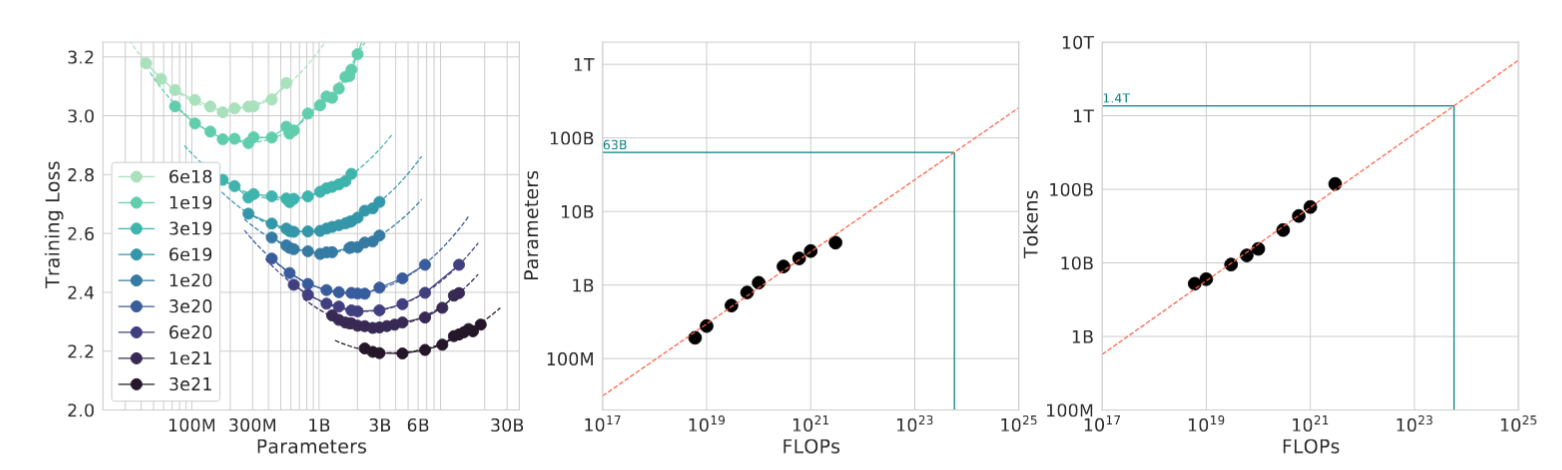
\includegraphics[width=\linewidth]{part1/visuals/isoflop.png}};
\begin{scope}[x={(plot.south east)},y={(plot.north west)},every node/.style={font=\scriptsize,inner sep=0pt}]
\fill[white] (.018,.30) rectangle (.040,.70);
\node[rotate=90] at (.031,.50) {训练损失};
\fill[white] (.331,.30) rectangle (.350,.70);
\node[rotate=90] at (.341,.50) {参数量};
\fill[white] (.654,.32) rectangle (.670,.68);
\node[rotate=90] at (.662,.50) {词元数};
\fill[white] (.12,0) rectangle (.28,.075);
\node at (.20,.028) {参数量};
\end{scope}
\end{tikzpicture}

    \caption{IsoFLOP 曲线 \citep{10.5555/3600270.3602446}。}
    \label{fig:isoflop}
\end{figure}

\paragraph{微调的扩展规律}
前述工作研究的是预训练如何扩展。这些扩展定律是否也支配微调？\citet{zhang2024when} 针对两种情形研究了这个问题：一种是更新模型全部权重的全模型微调；另一种是参数高效微调（parameter-efficient finetuning，PEFT），即冻结预训练权重，只训练少量新增参数，LoRA 就是这样的例子 \citep{hu2021lora}。对于计算预算而言，最相关的结论是：扩大\emph{基础模型}的规模，比收集更多微调数据更能提升微调性能，而增加 PEFT 的可训练参数则帮助不大。在实践中，如果某项任务的表现不佳，通常从更大的预训练模型开始，比扩大适配器或收集更多微调样本更有效。

\subsection{涌现能力}
大语言模型扩展中，一些最有趣的现象是\emph{涌现能力（emergent abilities）}：这些能力在小模型中并不存在，却会在模型规模或计算量越过某个阈值时突然出现 \citep{wei2022emergent}。例如，图~\ref{fig:emergent-abilities}~展示了多步推理、少样本翻译和专门的编程任务等例子。如果语言模型在达到某个规模之前，一直只有随机水平的表现，而超过这一规模后性能显著提升、远高于随机水平，那么通过少样本提示完成任务的能力就是涌现的。

\begin{figure}
    \centering
    % 八个面板的原始曲线、刻度和随机基线原样保留。
\begin{tikzpicture}
\node[anchor=south west,inner sep=0] (plot) at (0,0) {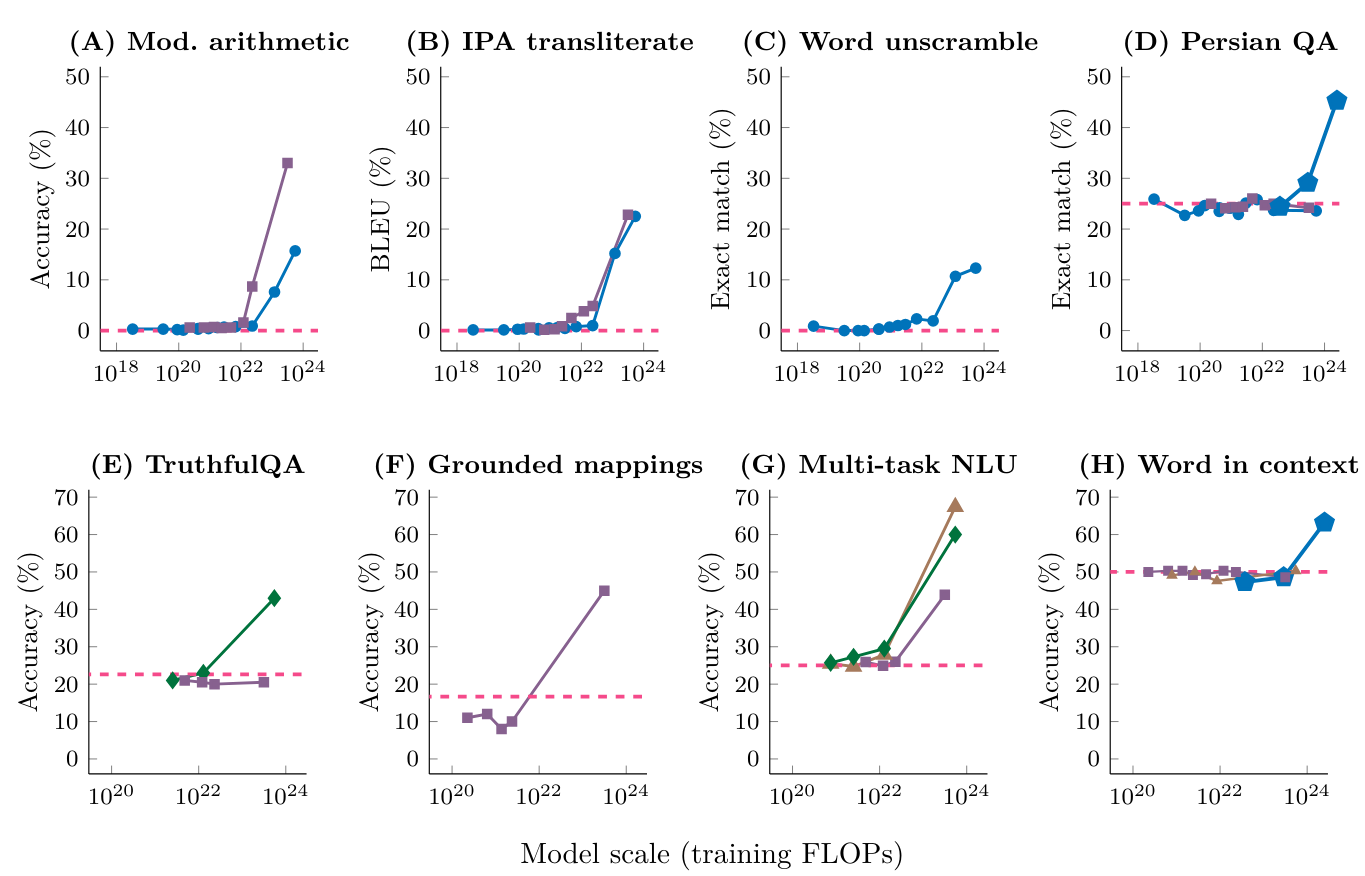
\includegraphics[width=.9\linewidth]{part1/visuals/emergent.png}};
\begin{scope}[x={(plot.south east)},y={(plot.north west)},every node/.style={font=\scriptsize,inner sep=0pt}]
\fill[white] (.04,.935) rectangle (.999,.99);
\node at (.150,.957) {(A) 模算术};
\node at (.404,.957) {(B) 国际音标转写};
\node at (.652,.957) {(C) 字母重排};
\node at (.900,.957) {(D) 波斯语问答};
\fill[white] (.04,.450) rectangle (.999,.492);
\node at (.145,.471) {(E) TruthfulQA};
\node at (.402,.471) {(F) 锚定映射};
\node at (.652,.471) {(G) 多任务自然语言理解};
\node at (.900,.471) {(H) 语境词义};
\foreach \xx/\txt in {.027/准确率（\%）,.278/BLEU（\%）,.528/精确匹配率（\%）,.778/精确匹配率（\%）}{
    \fill[white] (\xx-.015,.59) rectangle (\xx+.015,.86);
    \node[rotate=90] at (\xx,.727) {\txt};
}
\foreach \xx in {.019,.274,.525,.775}{
    \fill[white] (\xx-.015,.12) rectangle (\xx+.015,.39);
    \node[rotate=90] at (\xx,.255) {准确率（\%）};
}
\fill[white] (.34,0) rectangle (.68,.049);
\node at (.51,.024) {模型规模（训练 FLOPs）};
\end{scope}
\end{tikzpicture}

    \caption{少样本提示设置下涌现现象的八个例子，每个点对应一个不同的模型 \citep{wei2022emergent}。}
    \label{fig:emergent-abilities}
\end{figure}

不过，能力出现的突然性受到了质疑。\citet{schaeffer2023emergent} 认为，涌现能力可能是选择评估指标所造成的假象。例如，图~\ref{fig:emergent}~表明，不平滑的离散指标，例如准确率或精确匹配率，会出现陡然跳跃，毕竟它们本来就不平滑；但其底层指标，例如交叉熵损失或词元级概率，则在不同规模上遵循平滑、可预测的幂律。

\begin{figure}
    \centering
    % 原始两面板及数据保持不变；翻译标题、轴题和图例标题。
\begin{tikzpicture}
\node[anchor=south west,inner sep=0] (plot) at (0,0) {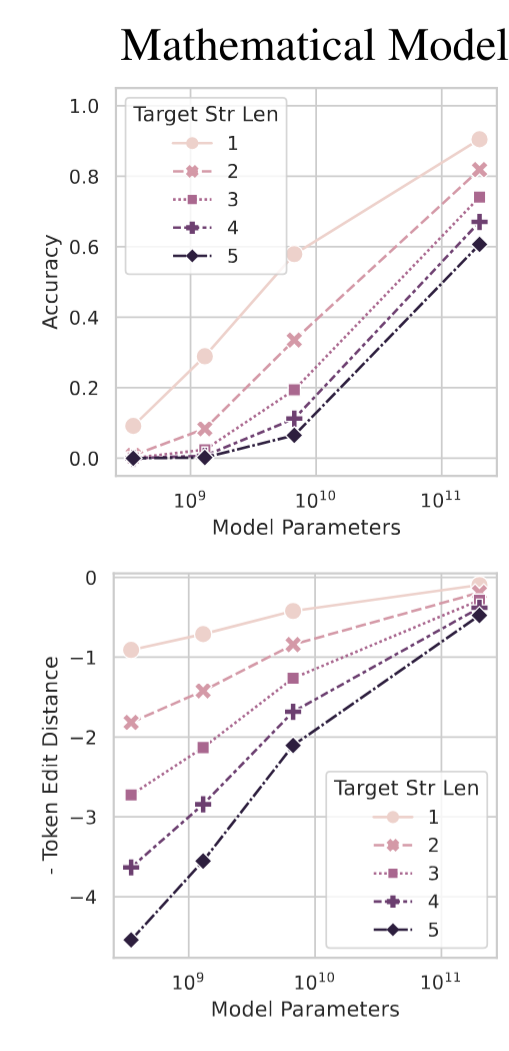
\includegraphics[width=.36\linewidth]{part1/visuals/token_edit.png}};
\begin{scope}[x={(plot.south east)},y={(plot.north west)},every node/.style={font=\scriptsize,inner sep=0pt}]
\fill[white] (.18,.932) rectangle (1,1);
\node[font=\small] at (.59,.966) {数学模型};
\fill[white] (.04,.61) rectangle (.13,.80);
\node[rotate=90] at (.09,.705) {准确率};
\fill[white] (.31,.480) rectangle (.92,.515);
\node at (.615,.497) {模型参数量};
\fill[white] (.25,.879) rectangle (.56,.91);
\node at (.405,.894) {目标字符串长度};
\fill[white] (.04,.15) rectangle (.13,.38);
\node[rotate=90] at (.09,.265) {负词元编辑距离};
\fill[white] (.31,.018) rectangle (.92,.055);
\node at (.615,.037) {模型参数量};
\fill[white] (.65,.235) rectangle (.97,.266);
\node at (.81,.251) {目标字符串长度};
\end{scope}
\end{tikzpicture}

    \caption{当评估指标由非线性指标（上图）改为平滑指标（下图）时，所声称的涌现能力便消失了 \citep{schaeffer2023emergent}。}
    \label{fig:emergent}
\end{figure}

\subsection{逆向扩展}
虽然大多数任务会随规模增大而改善，但有些任务呈现\emph{逆向扩展（inverse scaling）}，即更大的模型表现更差，或产生更强的偏差。如果某项任务中的干扰答案在语言建模目标下比正确答案的概率更高，就可能出现这种现象，使更大、也更有信心的模型持续选择错误选项 \citep{mckenzie2023inverse, michaelov-bergen-2023-emergent}。

逆向扩展的一个例子是\emph{忽略事后结果（hindsight neglect）}任务，它根据期望值测试某次下注是否值得。在期望值为正时，模型应当回答{\em 是}；期望值为负时，则应当回答{\em 否}。具体设置如下：模型只看到一些少样本示例，其中实际结果始终与期望值一致，也就是说，期望值为正时下注者赢钱，期望值为负时则输钱。随后，模型会被问到：对于一次期望值与实际结果不一致的下注，下注这一决定是否正确。忽略事后结果任务测试的是：当少样本示例的标签正确却具有误导性时，模型能否根据指令作出正确泛化。重复代数（Repetitive Algebra）任务则测试，在给定某种特定模式、标签正确的少样本示例时，模型会如何回答简单代数问题。图~\ref{fig:negative-scaling}~表明，模型起初的表现通常接近随机水平，但在训练计算量达到约 $10^{22}$ FLOPs 时，表现会降至随机水平以下。

\begin{figure}
    \centering
    % 数据点、连线与模型图例保留，中文仅覆盖原有英文说明。
\begin{tikzpicture}
\node[anchor=south west,inner sep=0] (plot) at (0,0) {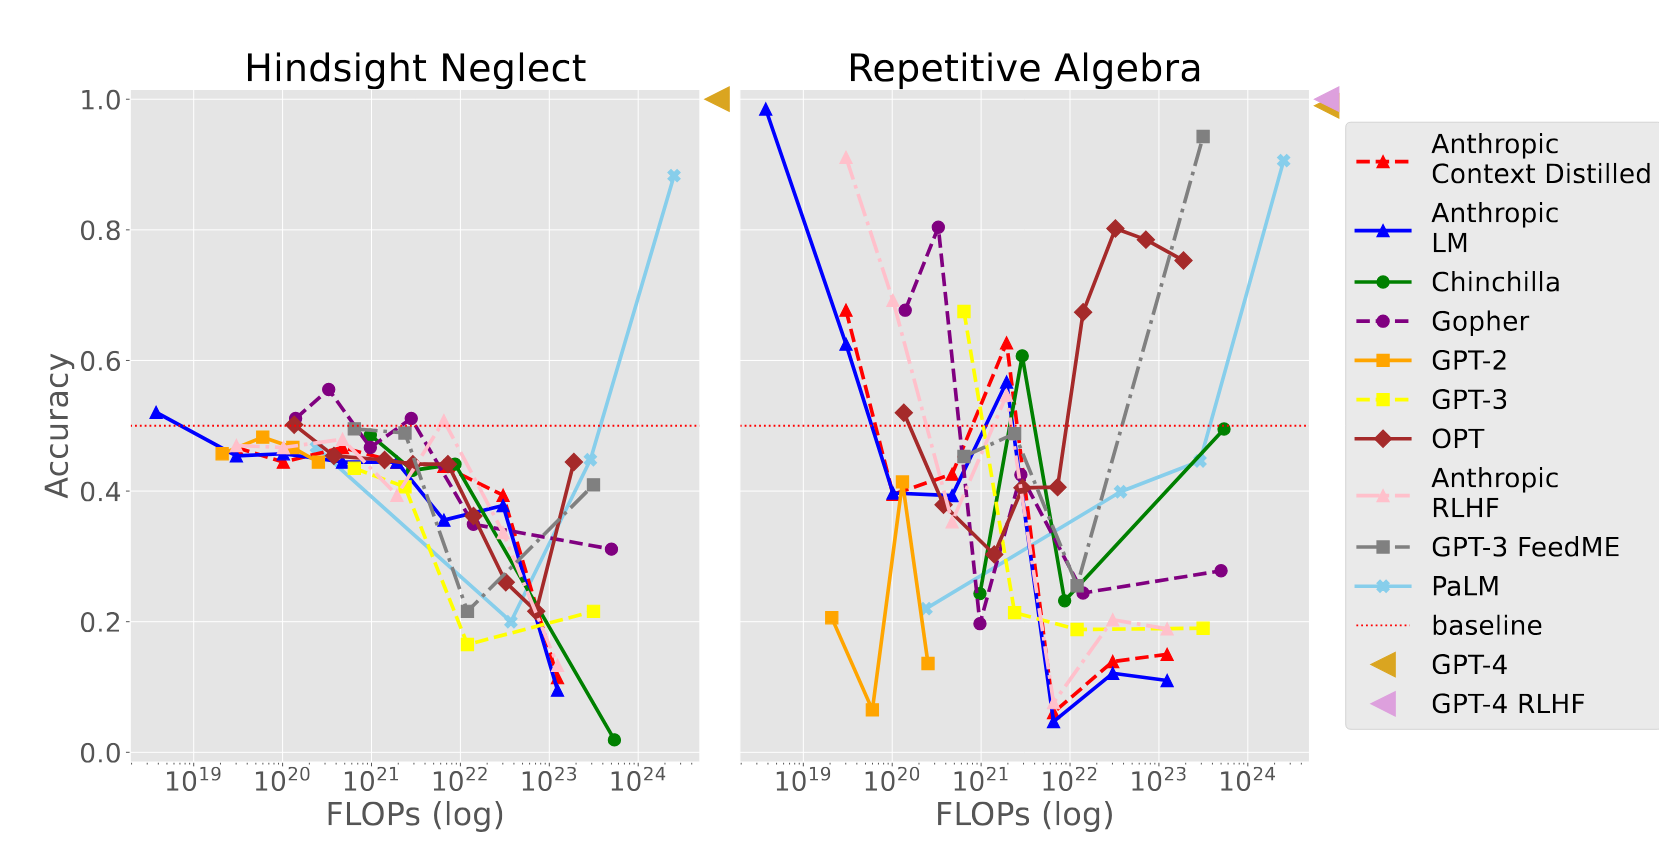
\includegraphics[width=.8\linewidth]{part1/visuals/negative_scaling.png}};
\begin{scope}[x={(plot.south east)},y={(plot.north west)},every node/.style={font=\scriptsize,inner sep=0pt}]
\fill[white] (.13,.90) rectangle (.78,.97);
\node[font=\small] at (.246,.927) {忽略事后结果};
\node[font=\small] at (.610,.927) {重复代数};
\fill[white] (.018,.32) rectangle (.045,.65);
\node[rotate=90] at (.032,.49) {准确率};
\fill[white] (.16,0) rectangle (.72,.065);
\node at (.247,.029) {FLOPs（对数）};
\node at (.610,.029) {FLOPs（对数）};
\fill[black!8] (.846,.775) rectangle (.985,.816);
\node at (.915,.795) {上下文蒸馏};
\fill[black!8] (.847,.245) rectangle (.955,.279);
\node at (.90,.263) {基线};
\end{scope}
\end{tikzpicture}

    \caption{忽略事后结果（左）与重复代数（右）任务的扩展行为 \citep{mckenzie2023inverse}。}
    \label{fig:negative-scaling}
\end{figure}

\subsection{顿悟}
顿悟（grokking）是统计学习理论中一个较近才被发现的悖论。按照这一理论的常规认识，用小数据集训练大模型时，模型会因记住样本而过拟合。而顿悟是指：继续训练这个过大的模型，在经历大量额外训练之后，模型突然找到一个能够泛化的解 \citep{power2022grokkinggeneralizationoverfittingsmall}。

顿悟现象最初是在模加法等小型算法任务中观察到的，但它表明，即使不增加数据集规模 $D$，仅仅增加训练步数，即进行超额训练，也可能带来从记忆到理解的质变，见图~\ref{fig:grokking}。

\begin{figure}
    \centering
    % 保留全部训练/测试损失曲线，只翻译文字。
\begin{tikzpicture}
\node[anchor=south west,inner sep=0] (plot) at (0,0) {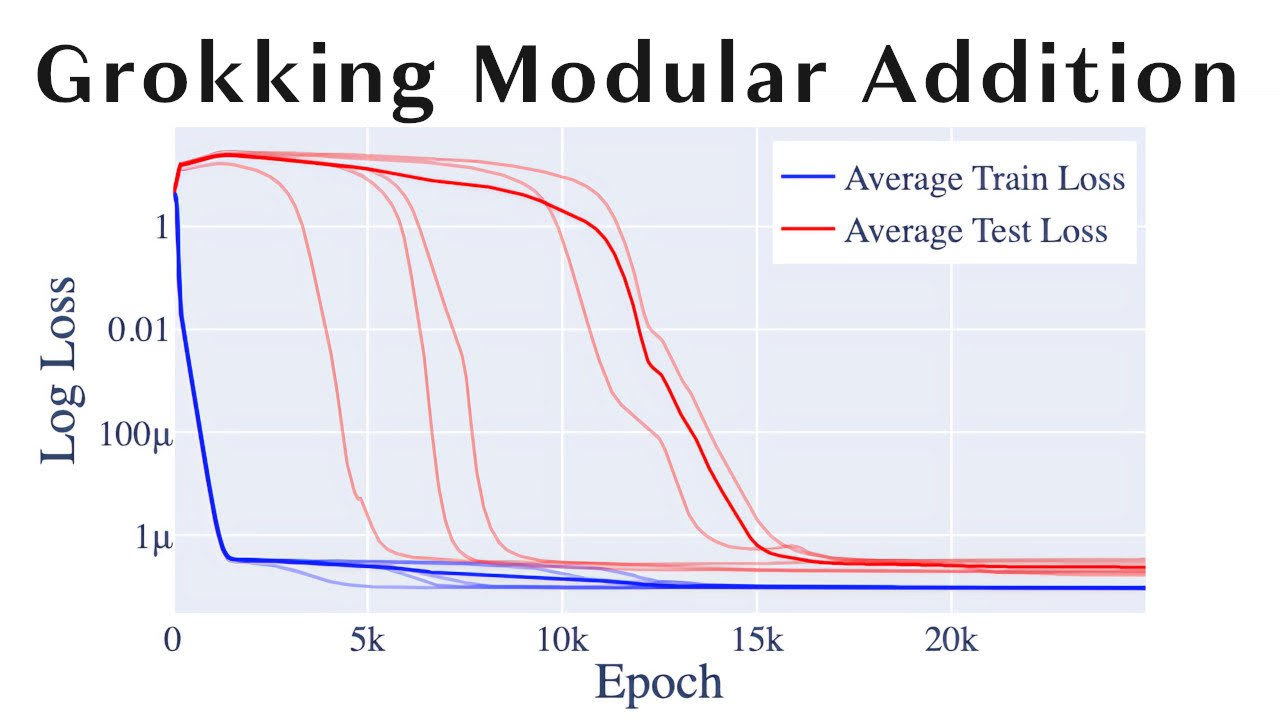
\includegraphics[width=.6\linewidth]{part1/visuals/Grokking_modular_addition.jpg}};
\begin{scope}[x={(plot.south east)},y={(plot.north west)},every node/.style={font=\scriptsize,inner sep=0pt}]
\fill[white] (0,.85) rectangle (1,1);
\node[font=\small] at (.50,.925) {模加法中的顿悟};
\fill[white] (0,.29) rectangle (.068,.66);
\node[rotate=90] at (.047,.475) {对数损失};
\fill[white] (.43,0) rectangle (.67,.08);
\node at (.55,.041) {训练轮次};
\fill[white] (.655,.72) rectangle (.885,.79);
\node at (.77,.755) {平均训练损失};
\fill[white] (.655,.65) rectangle (.885,.715);
\node at (.77,.682) {平均测试损失};
\end{scope}
\end{tikzpicture}

    \caption{模加法任务中，早期对训练集的记忆（蓝色）与后期泛化（红色，即顿悟）的对比 \citep{nanda2023progress}。}
    \label{fig:grokking}
\end{figure}

图中展示了一道数据墙：起初，随着数据耗尽，它限制了扩展 \citep{villalobos2024position}；但后来，在经历大量额外训练之后，模型顿悟出一个能够泛化的解。

顿悟与语言建模密切相关，因为为了满足下一代模型遵循 Chinchilla 扩展规律所需的数据量 $D$，互联网中的高质量人类文本正迅速耗尽。由于这些内在限制，研究者开始探索简单增加 $D$ 之外的途径。作为替代，我们可以考察多种新的前沿方向：
(1) 更高的架构效率，例如混合专家模型；
(2) 推理阶段扩展，例如给予模型更多推理计算量来{\em 思考}，OpenAI 的 o 系列就是这样的例子；
(3) 合成数据生成（第~\ref{chap:synthetic-data}~章）。

\section{小语言模型}
\label{sec:small-models}
随着计算与数据需求不断增长，人们对\emph{小语言模型（small language models，SLMs）}的兴趣也越来越浓厚。这类模型规模足够小，能够在消费级硬件，乃至移动设备或边缘设备上运行，同时保持较高性能。开发这类模型时，往往会使用一些技术来优化效率，而不牺牲过多性能。

为了理解这类模型的部署环境，有必要对常见的计算基础设施进行分类：
\begin{itemize}
    \item 数据中心：高性能 GPU，例如 NVIDIA H100，以及 TPU，主要用于大模型的{\em 预训练}和承载高吞吐量的推理 API。

    \item 消费级硬件：标准桌面 GPU 与高端 CPU，个人用户能够以可承受的成本在这些硬件上{\em 微调}小语言模型，或在本地运行它们。

    \item 边缘设备：手机、物联网设备和笔记本电脑。这些设备越来越多地配备神经处理单元（neural processing unit，NPU），专门用于低功耗、高效率的设备端{\em 推理}。
\end{itemize}

为了让模型适应后两类资源受限的环境，优化技术主要着眼于提高吞吐量、降低延迟、减少内存占用，以及提高样本效率。实现这些目标的技术可以分为两类：(1) 以模型为中心的优化，针对模型架构及其优化方法；(2) 以数据为中心的优化，针对用于训练模型的数据。下面将讨论这两类技术。

\subsection{以模型为中心的优化}
首先讨论以模型为中心的优化技术。
我们将介绍以下技术，它们能够高效地训练较小模型，同时仍然保持较高的任务性能。
以模型为中心的技术，既可以着眼于预训练或微调，也可以着眼于推理。

\subsubsection{降低预训练成本}

\paragraph{参数高效微调（PEFT）}

{\em 低秩适配（Low-Rank Adaptation，LoRA）}等方法 \citep{hu2021lora}，只需训练大模型中极小一部分参数，通常为 $<1$\%，就能使其适应新任务 \citep{lialin2023scaling}。其关键观察是，微调过程中学到的权重更新具有较低的{\em 内在秩（intrinsic rank）}：虽然预训练权重矩阵
$W_0 \in \mathbb{R}^{d \times k}$
是满秩的，但使它适应新任务所需的变化 $\Delta W$，可以用一个低秩矩阵很好地近似。LoRA 不直接更新 $W_0$，而是将其冻结，并把更新表示为两个小矩阵的乘积：
\begin{equation}
    W = W_0 + \Delta W = W_0 + B A, \qquad B \in \mathbb{R}^{d \times r}, \;\; A \in \mathbb{R}^{r \times k}
\end{equation}
其中，秩 $r \ll \min(d, k)$。对于输入 $x$，修改后的前向传播为
\begin{equation}
    h = W_0 x + \frac{\alpha}{r}\, B A x,
\end{equation}
其中，$\alpha$ 是控制更新幅度的常数缩放因子，作用与标准训练中的学习率大致相似。图~\ref{fig:lora}~展示了这一过程。我们只计算 $A$ 和 $B$ 的权重更新，将可训练参数量从 $d \times k$ 降为 $r(d + k)$。初始化时，$A$ 从随机高斯分布中抽取，$B$ 则设为零，因此 $\Delta W = 0$，训练从预训练模型的状态开始。训练结束后，$\Delta W$ 可以直接合并回 $W_0$，所以 LoRA 不会增加推理延迟；同一个基础模型还可以配合许多小型、可替换的任务专用适配器提供服务。

\begin{figure}[t]
    \centering
    % 按随附 part1/visuals/lora.png 重绘，保留原图的 d x d 特例与初始化符号。
\resizebox{.58\linewidth}{!}{%
\begin{tikzpicture}[x=1cm,y=1cm,
    every node/.style={font=\normalsize,align=center,inner sep=3pt},
    flow/.style={-{Stealth[length=3mm,width=2.4mm]},line width=1.1pt,draw=blue!55!black}]
\filldraw[fill=blue!55!white,draw=black,line width=1pt] (0,1.6) rectangle (3.6,5.2);
\node[text=white,font=\large] at (1.8,4.1) {预训练权重};
\node[text=white,font=\large] at (1.8,2.7) {$W\in\mathbb{R}^{d\times d}$};
\filldraw[fill=orange!85!black,draw=black,line width=1pt] (4,1.6) -- (7.6,1.6) -- (6.5,2.9) -- (5.1,2.9) -- cycle;
\node[text=white,font=\large] at (5.8,2.05) {$A=\mathcal{N}(0,\sigma^2)$};
\filldraw[fill=orange!85!black,draw=black,line width=1pt] (4,5.2) -- (7.6,5.2) -- (6.5,3.9) -- (5.1,3.9) -- cycle;
\node[text=white,font=\large] at (5.8,4.5) {$B=0$};
\filldraw[fill=yellow!55,draw=black,line width=1pt] (2.0,0) rectangle (5.6,.35);
\node[font=\Large,anchor=east] at (1.9,.18) {$x$};
\filldraw[fill=yellow!55,draw=black,line width=1pt] (2.0,6.45) rectangle (5.6,6.8);
\node[font=\Large,anchor=east] at (1.9,6.62) {$h$};
\draw[flow] (2.45,.52) -- (1.8,1.4);
\draw[flow] (5.05,.52) -- (5.8,1.4);
\draw[flow] (1.8,5.4) -- (2.7,6.2);
\draw[flow] (5.8,5.4) -- (4.9,6.2);
\node[text=blue!55!black,font=\Huge] at (3.8,5.95) {$+$};
\draw[decorate,decoration={brace,amplitude=4pt},draw=blue!55!black] (2.0,.65) -- node[above=4pt,text=black,font=\large] {$d$} (5.6,.65);
\draw[decorate,decoration={brace,amplitude=4pt},draw=blue!55!black] (5.1,3.15) -- node[above=4pt,text=black,font=\large] {$r$} (6.5,3.15);
\end{tikzpicture}%
}

    \caption{低秩适配的重参数化 \citep{hu2021lora}。微调时只训练 $A$ 和 $B$。}
    \label{fig:lora}
\end{figure}

\paragraph{架构创新}
第二类技术直接改变模型架构，使模型运行成本更低，而不是事后压缩一个固定架构。分组查询注意力与混合专家模型是两个影响广泛的例子。

\textit{分组查询注意力（Grouped-Query Attention，GQA）} \citep{ainslie-etal-2023-gqa} 针对的是自回归解码中的内存带宽瓶颈。在标准的\emph{多头注意力（multi-head attention，MHA）}中，每个查询头都有自己的键矩阵和值矩阵，计算注意力分数时需要用到所有这些矩阵。另一个极端是\emph{多查询注意力（multi-query attention，MQA）}，它让所有查询头共享一个键／值头，从而减少计算量，但可能损害表达能力和训练稳定性。GQA 介于二者之间：将查询头分为 $g$ 组，同组的所有头共享一个键／值头。当 $g = 1$ 时，它等价于 MQA；当 $g$ 等于头的总数时，它等价于 MHA，因此 $g$ 在质量与内存占用之间起着权衡作用。GQA 常与第~\ref{sec:small-models}~节接下来讨论的 KV 缓存优化结合使用，如今已成为许多开放权重模型默认采用的注意力变体。

\textit{混合专家（Mixture of Experts，MoE）} \citep{shazeer2017outrageouslylargeneuralnetworks} 将参数总量与每个词元所消耗的计算量分离。MoE 层不再为每一层配置单个稠密前馈模块，而是包含多个并行的“专家”子网络，以及一个轻量的\emph{门控网络（gating network）}，也称路由器；对于每个词元，它只激活少数几个专家，通常是得分最高的 $1$ 个或 $2$ 个。由于只有选中的专家执行计算，即使参数总量、因而模型的总体容量增长一个或更多数量级，每个词元的成本仍接近单个稠密模块的成本 \citep{JMLR:v23:21-0998}。

正是这种\emph{稀疏激活（sparse activation）}，使 Mixtral 和许多近期的前沿系统能够拥有数千亿总参数，却只为每个词元激活其中一小部分。相应的权衡有三点：(1) 所有专家仍必须驻留内存；(2) 必须在专家之间平衡负载，通常借助辅助损失，以免某个专家被过度使用或使用不足；(3) 路由会增加工程复杂度。图~\ref{fig:moe}~展示了 MoE 架构。其中采用 top-$k$ 路由机制，并设置 $k=2$，门控函数根据路由器的输出，为每个词元选择得分最高的两个前馈网络（FFN）专家。选中的专家并行求值，再通过加权求和汇总其输出 \citep{zhang2025mixtureexpertslargelanguage}。

\begin{figure}[t]
    \centering
    % 依照随附 part1/visuals/moe.png 重绘。路由权重逐项保留；不重新归一化。
\resizebox{\linewidth}{!}{%
\begin{tikzpicture}[x=1cm,y=1cm,
    every node/.style={font=\small,align=center,inner sep=2pt},
    flow/.style={-{Stealth[length=2mm,width=1.5mm]},line width=.7pt},
    residual/.style={-{Stealth[length=2mm,width=1.5mm]},line width=.7pt,rounded corners=2mm},
    norm/.style={draw=red!65!black,fill=red!18,rounded corners=1mm,minimum height=.4cm},
    attention/.style={draw=black!70,fill=yellow!30,rounded corners=1mm,minimum height=.4cm},
    expert/.style={draw=black,fill=violet!30,rounded corners=.6mm,minimum width=.5cm,minimum height=.3cm,font=\fontsize{6.8pt}{8pt}\selectfont,inner sep=1pt},
    router/.style={draw=green!55!black,fill=green!15,rounded corners=1mm,minimum height=.4cm},
    weight/.style={font=\scriptsize,fill=blue!5,inner sep=1pt}]

% 左：仅解码器 Transformer 中的 MoE 层。
\node[font=\bfseries\small,text=blue!65!black] at (1.6,7.9) {仅解码器 Transformer\\上的 MoE 架构};
\node[font=\large] (xin) at (1.6,2.3) {$x$};
\node[attention,minimum width=2.9cm] (sa) at (1.6,3.0) {自注意力};
\node[norm,minimum width=2.9cm] (n1) at (1.6,3.85) {相加与归一化};
\node[draw=blue!65!black,fill=blue!15,rounded corners=1mm,minimum width=2.9cm,minimum height=.4cm] (moe) at (1.6,4.7) {MoE 层};
\node[norm,minimum width=2.9cm] (n2) at (1.6,5.55) {相加与归一化};
\node[font=\large] (yout) at (1.6,6.4) {$y$};
\draw[flow] (xin) -- (sa);
\draw[flow] (sa) -- (n1);
\draw[flow] (n1) -- (moe);
\draw[flow] (moe) -- (n2);
\draw[flow] (n2) -- (yout);
\draw[dashed] (3.05,3.0) -- (4.55,1.5);
\draw[dashed] (3.05,5.55) -- (4.55,7.3);

% 右：四个词元各自路由至得分最高的两个专家。
\filldraw[draw=blue!55!black,fill=blue!5,rounded corners=4mm,line width=1.2pt] (4.85,2.65) rectangle (17.45,6.65);
\node[attention,minimum width=10.8cm] (fullsa) at (11.15,1.25) {自注意力};
\node[norm,minimum width=10.8cm] (fulln1) at (11.15,2.1) {相加与归一化};
\node[norm,minimum width=10.8cm] (fulln2) at (11.15,7.1) {相加与归一化};

\foreach \i/\xx/\c in {1/6.6/red,2/9.7/yellow,3/12.8/green,4/15.9/blue}{
    \foreach \j in {0,1,2,3,4}{
        \pgfmathtruncatemacro{\tone}{20+13*\j}
        \filldraw[fill=\c!\tone,draw=\c!60!black,line width=.3pt] (\xx-.45+.18*\j,-.25) rectangle ++(.18,.2);
        \filldraw[fill=\c!\tone,draw=\c!60!black,line width=.3pt] (\xx-.45+.18*\j,7.88) rectangle ++(.18,.2);
    }
    \node[font=\large] (pos\i) at (\xx,.45) {$\oplus$};
    \draw[flow] (\xx,-.03) -- (pos\i.south);
    \draw[flow] (pos\i.north) -- (\xx,1.05);
    \draw[flow] (\xx,1.45) -- (\xx,1.9);
    \draw[flow] (\xx,2.3) -- (\xx,3.25);
    \draw[flow] (\xx,7.3) -- (\xx,7.86);
    \foreach \j/\dx in {1/-.9,2/-.3,3/.3,4/.9}{
        \node[expert] (e\i\j) at (\xx+\dx,5.4) {FFN\j};
    }
    \node[font=\large] (sum\i) at (\xx,6.1) {$\otimes$};
    \draw[flow] (sum\i.north) -- (\xx,6.9);
}
\node[anchor=east,font=\scriptsize\bfseries] at (6.0,-.15) {词元嵌入};
\node[anchor=east,font=\scriptsize] at (6.05,.45) {位置嵌入};
\node[router,minimum width=1.7cm,minimum height=1.0cm,font=\fontsize{8pt}{9pt}\selectfont] (r1) at (6.6,3.28) {路由器：带 softmax\\的前馈网络\\$k=2$};
\node[router,minimum width=1.2cm] (r2) at (9.7,3.45) {路由器};
\node[router,minimum width=1.2cm] (r3) at (12.8,3.45) {路由器};
\node[router,minimum width=1.2cm] (r4) at (15.9,3.45) {路由器};

% 路由得分的小柱状示意逐列对应原图，仅表达原有概率权重。
\foreach \xx/\ha/\hb/\hc/\hd in {6.6/.63/.14/.22/.07,9.7/.28/.12/.58/.24,12.8/.08/.59/.24/.30,15.9/.26/.12/.61/.34}{
    \draw[draw=blue!55!black,fill=blue!15] (\xx-.28,3.93) rectangle ++(.12,\ha);
    \draw[draw=blue!55!black,fill=blue!15] (\xx-.14,3.93) rectangle ++(.12,\hb);
    \draw[draw=blue!55!black,fill=blue!15] (\xx,3.93) rectangle ++(.12,\hc);
    \draw[draw=blue!55!black,fill=blue!15] (\xx+.14,3.93) rectangle ++(.12,\hd);
}
\node[anchor=west,font=\scriptsize\bfseries] at (5.7,6.45) {汇总};
\draw[flow] (6.4,4.35) to[out=150,in=-90] node[weight,pos=.55,left] {$0.7$} (e11.south);
\draw[flow] (6.7,4.2) to[out=85,in=-90] node[weight,pos=.45,right] {$0.2$} (e13.south);
\draw[flow] (9.55,4.35) to[out=150,in=-90] node[weight,pos=.55,left] {$0.22$} (e21.south);
\draw[flow] (9.8,4.2) to[out=85,in=-90] node[weight,pos=.45,right] {$0.6$} (e23.south);
\draw[flow] (12.65,4.35) to[out=95,in=-90] node[weight,pos=.5,left] {$0.55$} (e32.south);
\draw[flow] (12.95,4.2) to[out=30,in=-90] node[weight,pos=.55,right] {$0.2$} (e34.south);
\draw[flow] (15.75,4.35) to[out=95,in=-90] node[weight,pos=.5,left] {$0.2$} (e43.south);
\draw[flow] (16.05,4.2) to[out=30,in=-90] node[weight,pos=.55,right] {$0.5$} (e44.south);
\foreach \i/\a/\b in {1/1/3,2/1/3,3/2/4,4/3/4}{
    \draw[flow] (e\i\a.north) -- (sum\i.south west);
    \draw[flow] (e\i\b.north) -- (sum\i.south east);
}
\draw[flow,dashed] (r1.west) to[out=180,in=180,looseness=1.5] (sum1.west);
\draw[flow,dashed] (r2.west) to[out=180,in=180,looseness=1.5] (sum2.west);
\draw[flow,dashed] (r3.west) to[out=180,in=180,looseness=1.5] (sum3.west);
\draw[flow,dashed] (r4.east) to[out=0,in=0,looseness=1.5] (sum4.east);

% 两条残差支路与原图一致。
\draw[residual] (15.9,.7) -- (5.15,.7) -- (5.15,2.1) -- (5.75,2.1);
\draw[residual] (15.9,2.5) -- (4.5,2.5) -- (4.5,7.1) -- (5.75,7.1);
\end{tikzpicture}%
}

    \caption{在仅解码器 Transformer 上构建的稀疏门控混合专家（MoE）架构示意图 \citep{zhang2025mixtureexpertslargelanguage}。}
    \label{fig:moe}
\end{figure}

\paragraph{知识蒸馏}
知识蒸馏（knowledge distillation）使用大型教师模型来训练较小的学生模型，鼓励学生匹配教师的输出分布 \citep{gu2023minillm, xu2024survey}。关键在于，学生学习的是教师完整的\emph{软}概率，通常通过温度参数加以软化，而不只是单个正确答案。这些软目标包含更丰富的信息，例如，教师认为哪些错误答案也有一定可能性。这让学生能以远小于教师的规模，达到接近教师的质量。同样的思想也支撑着下文将讨论的合成数据生成：前沿模型实际上充当教师，为较小的学生模型生成高质量训练数据。

\subsubsection{降低推理成本}
模型训练完成后，还可以进一步优化，以便在推理阶段部署。训练阶段的技术着眼于降低模型的生产成本，而推理阶段的技术则针对\emph{使用}模型的成本：吞吐量，即每秒生成的词元数；延迟，即生成首个词元以及后续每个词元所需的时间；以及处理请求所需的内存占用。下面讨论几种常用于降低推理成本的技术，它们对大模型和小模型都适用。

\paragraph{键值（KV）缓存} 在自回归生成中，模型每次生成一个词元，而每个新词元都要注意到此前的全部词元。如果每一步都重新计算整个上下文的注意力键和值，计算成本会呈二次增长。不过，在预测一个新词元时，已有上下文并没有改变。我们可以将过去词元的键向量和值向量保存在\emph{KV 缓存（KV cache）}中并重复使用，而不必重新计算注意力所需的值。这将每一步的注意力计算变为线性成本的查找。它是让解码切实可行的基础优化，但也有代价：缓存会随序列长度与批量大小线性增长，在长上下文中很快就会占据内存使用量的主要部分。这一问题既推动了前述架构选择，即 GQA 与 MQA 通过在查询头之间共享键／值头来缩小缓存，也催生了 \emph{PagedAttention} 等专门的内存管理方案。后者将缓存存储在不连续的块中，以减少碎片并提高服务吞吐量 \citep{kwon2023efficient}。

\paragraph{剪枝} 一种更激进的缩小模型方法，是考虑移除神经网络中冗余或不太重要的连接 \citep{ma2023llm}。剪枝（pruning）可以是\emph{非结构化}的，即将单个权重置零；也可以是\emph{结构化}的，即移除整个神经元、注意力头或层。后者能在标准硬件上带来实际加速，而前者需要支持稀疏计算的内核，才能实现其收益。

\paragraph{量化} 推理阶段节省内存的另一种方法，是减小需要加载到内存中的矩阵所占的空间。除了缩小矩阵维度，我们也可以降低权重元素的精度，例如从 16 位降到 8 位或 4 位数值。这会显著减少内存占用，并加快推理。不过，原则上，精度更低也意味着性能更低。同样的思想还可以应用于 KV 缓存本身，使长上下文能够留在内存中。量化（quantization）是一种经常使用的方法 \citep{dettmers2022gpt3, dettmers2023case, xiao2023smoothquant}。

另一种选择是采用\emph{混合精度（mixed precision）}模式，而不是将所有权重转换成相同精度。这类模式为计算的不同部分使用不同的数值精度，以平衡速度与稳定性 \citep{micikevicius2017mixed}。这种方法可能因数值不稳定而产生非确定性结果 \citep{yuan2025understanding}。

\paragraph{推测解码} 优化推理效率的一项关键技术是\emph{推测解码（speculative decoding）} \citep{leviathan2023fast}。这种方法使用一个小型草稿模型快速生成多个词元，再由更大的目标模型并行验证。它可以在不牺牲大模型质量的前提下加快推理，最高可达到 2--3 倍加速，从而有效利用扩展曲线上的不同位置。

\subsection{以数据为中心的优化}
除了以模型为中心的方法，文献还强调，训练高效模型时，数据质量与整理往往比数据集规模更重要 \citep{luo-etal-2025-survey}。如果使用经过精心整理的高质量数据来训练，小模型也能够表现良好。因此，除了高效的模型架构，还需要制定良好的数据配方。以数据为中心的技术大体分为两类：从更广泛的数据池中\emph{选择}最有用的部分，以及在优质数据稀缺时\emph{生成}新的合成数据。

\subsubsection{数据选择与整理}
越来越多的研究表明，与其使用所有可获得的文本进行训练，不如仔细选择\emph{用哪些}数据训练，以及各类数据的比例；在相同计算预算下，这样可以得到更好的模型。对于预训练，NVIDIA 的 \emph{CLIMB} 框架 \citep{diao2026nemotron} 将大型语料库嵌入到语义空间中，进行聚类，然后迭代搜索使代理模型损失最小的数据混合方案。由此得到的 \emph{ClimbMix} 数据集包含 4000 亿词元，使一个参数量不足十亿的模型，胜过在规模大得多、但未经筛选的语料库上训练的同类模型。同样的原则也适用于微调阶段：\emph{LIMA} \citep{zhou2023lima} 表明，只用 $1{,}000$ 对精心整理的提示与回答进行监督微调，就足以得到指令遵循能力很强的模型。这支持了这样一种观点：大部分知识在预训练期间获得，对齐主要是教会模型期望的回答\emph{风格}。

\subsubsection{合成数据获取}
如果不存在合适的数据，就可以生成数据。微软 Phi 系列等模型采用的 {\em Textbooks Are All You Need} 方法 \citep{gunasekar2024textbooks} 表明，使用干净、达到教科书质量的合成数据训练，可以让一个仅有 13 亿参数的较小模型，胜过规模十倍于它的模型。

这类训练流程通常依靠前沿模型生成数据，结合{\em 大语言模型裁判（LLM-as-a-judge）}评分，筛选最准确、最具教学价值的样本，并严格执行\emph{去污染（decontamination）}，以确保合成数据不会泄露基准测试集、虚增报告的性能。这种方法对于推理数据尤其有价值：通过在较大模型生成的逐步推理轨迹上训练，可以将复杂的问题求解技能蒸馏到较小的架构中（另见第~\ref{chap:reasoning}~章）\citep{muennighoff2025s1, arora2026training}。

\subsubsection{高样本效率学习}
除合成数据以外，研究者也越来越关注模型如何更高效地从有限、贴近自然环境的数据中学习。\emph{BabyLM Challenge} 等项目 \citep{warstadt-etal-2023-findings} 专注于在严格的数据约束下训练模型，例如只使用 1000 万至 1 亿词元。这与人类儿童在早期发育中接收的语言输入量相近，既推动了高样本效率架构的创新，也为符合认知实际的语言习得提供了见解。

\subsection{常见模型}
在概览了改进技术之后，再考察常见的大模型与小模型如何在实践中运用这些技术，会很有帮助。模型通常按照开放程度分类：封闭权重的专有模型只提供 API；开放权重模型发布训练后的参数；开源模型则进一步共享训练数据与代码。实际上，开放性是程度问题，而不是严格的类别之分，因此也可以进一步使用开放性指数来评定透明度 \citep{artificialanalysis_openness}。大多数开放模型都可以在 Hugging Face 等仓库中找到。

下面简要介绍一些最常见的开放权重模型，以及它们为实现高效运行所采用的技术。这些模型在设计上力求高效，使其足以在消费级硬件上运行。这不是一份详尽的清单，而是选取了写作时一些具有影响力的模型，以展示效率技术及其规模的发展趋势。
\begin{description}[font=\bfseries]
    \item[Phi 系列] \citep{abdin2024phi3technicalreporthighly}。Phi 系列是能力较强的小语言模型，其效率足以支持在移动设备上本地运行。Phi 模型背后的核心创新是以数据为中心的训练方法。微软将经过严格筛选的高质量网页数据，与较大模型生成的合成数据结合起来并加以整理。这使小模型，例如具有 38 亿参数的 \texttt{Phi-3-mini}，能够表现出色，在推理能力上与 GPT-3.5 和 Mixtral 等大得多的模型相媲美。
    \item[Gemma 系列] \citep{gemmateam2024gemmaopenmodelsbased}。Google 强调，Gemma 模型继承了 Gemini 强大的通用能力，特别是在文本、推理和编程方面，同时在各自规模类别中推进了最先进水平；但外界对其训练方法或数据知之甚少。
    \item[OLMo 家族] \citep{olmo2025olmo3}。OLMo（Open Language Model）家族由 Allen Institute for AI 开发，目标是成为完全开源的模型。OLMo 项目开放了包含代码与数据的完整训练流程：预训练数据集 Dolma、训练和评估代码、训练日志，以及中间检查点。这种透明度使研究者能够研究训练动态、数据影响和算法偏差。
    \item[Qwen 系列] \citep{bai2023qwentechnicalreport}。Qwen 家族是一组高性能基础模型和指令微调模型，范围从不足十亿参数的稠密模型，一直到大型混合专家（MoE）架构。它们以多语言能力，以及在数学、编程和逻辑推理基准测试中的表现而著称。
    \item[OpenELM] \citep{mehta2024openelmefficientlanguagemodel}。Apple 的高效语言模型家族旨在边缘设备上高效运行。其逐层扩展策略在靠近输入的层中使用较小的潜在维度，在靠近输出的层中则增大维度。这使模型能够以较低参数量实现较高准确率。
    \item[gpt-oss] \citep{openai2025gptoss120bgptoss20bmodel}。OpenAI 发布了两个开放权重推理模型，采用高效的混合专家架构，并针对智能体能力进行了优化。
    \item[Mixtral 系列] \citep{jiang2024mixtralexperts}。这些模型，例如 Mixtral 8x7B，在开放权重生态中推广了稀疏混合专家（Sparse Mixture-of-Experts，SMoE）架构。它们允许模型拥有很大的参数总量，却只在推理时激活少量参数，以最大限度地提高效率。
    \item[Llama 系列] \citep{grattafiori2024llama3herdmodels}。Meta 的 Llama 模型已得到广泛使用。它们在大型数据集上训练，Llama 3 的训练词元数最高达到 15 万亿；模型规模从适合边缘设备的小型模型，一直到具有 4050 亿参数的大型前沿模型。这些模型为开放模型的扩展定律树立了标准，并促成了一个包含微调模型及衍生模型的生态。
    \item[DeepSeek] \citep{deepseekai2025deepseekv3technicalreport}。DeepSeek-V3 是一个大型混合专家模型，总参数量为 6710 亿，每个词元激活 370 亿参数，以训练稳定性而著称。它将用于压缩键值缓存的多头潜在注意力（Multi-head Latent Attention，MLA），与无辅助损失的专家负载均衡策略相结合，并采用 FP8 混合精度训练，以较小计算成本达到前沿水平。该系列还包括 DeepSeek-R1 推理模型。
    \item[GLM] \citep{glm5team2026glm5vibecodingagentic}。GLM（General Language Model）家族由智谱 AI 开发，其基础是在训练早期形成、并在整个训练过程中保留的强大推理能力。近期版本针对智能体工作流程与软件工程进行优化，着眼于工具使用和代码生成的性能，而不仅是文本补全。
    \item[Pythia] \citep{biderman2023pythia}。EleutherAI 的 Pythia 是一组参数量从 7000 万到 120 亿的模型，旨在支持对训练动态和扩展规律的研究。所有模型都以相同顺序在相同数据上训练，并且每个模型都发布了中间检查点，从而能够在受控条件下研究能力、记忆和偏差如何在训练过程中出现。
    \item[BLOOM] \citep{workshop2023bloom176bparameteropenaccessmultilingual}。BLOOM 是 BigScience 协作研究项目开发的一个具有 1760 亿参数的开放获取模型。它在 ROOTS 语料库上训练，覆盖 46 种自然语言和 13 种编程语言，是最早优先考虑多语言覆盖与完全开放的大规模模型之一，并以 Responsible AI License 发布。
    \item[SmolLM] \citep{allal2025smollm}。Hugging Face 的 SmolLM 是一个紧凑模型家族，包含 1.35 亿、3.6 亿和 17 亿参数的模型，与 Phi 系列相似，旨在实现高效的设备端部署。其性能来自数据整理：它使用 SmolLM-Corpus 训练，该语料库结合了高质量网页数据、Python 代码示例，以及用 Mixtral 合成的教科书和故事。
\end{description}

\section{推理阶段计算量}
\label{sec:inference-time}

传统扩展定律着眼于\textit{训练阶段}计算量与性能之间的关系。较近的研究将其中一部分计算负担转移到推理阶段，即\emph{推理阶段扩展（inference-time scaling）}，也称测试阶段计算 \citep{muennighoff2025s1}。模型不再将全部计算量用在训练期间，而是允许自己在推理阶段思考更长时间。为了获得更高质量的答案，这种投入用生成的词元数或探索的推理路径数来衡量。因此，优化吞吐量，即每秒生成的词元数，变得格外重要：生成词元越快，模型就越能在相同时间内进行更多推理。

增加以词元数衡量的推理阶段预算，可以显著提升能力 \citep{du2024debate}；近期工作表明，最优地分配测试阶段计算量，可以让较小模型在困难推理任务中胜过较大模型 \citep{snell2024scaling}。不过，这些收益并非必然，取决于任务以及所采用的具体搜索或验证策略 \citep{stechly2023gpt}。除了性能以外，这种转变也重新提出了一个更广泛的问题：大语言模型究竟属于何种系统？我们将在第~\ref{chap:reasoning}~章详细讨论。

\section{可持续语言模型}
\label{sec:sustainable}
大语言模型训练与部署的庞大规模，对环境和经济都有重大影响。人工智能训练与推理的能源消耗很大，
随之而来的冷却用水，也给供水管网带来了压力 \citep{10.1145/3724499, jegham2025hungryaibenchmarkingenergy}。直到近年，测量训练的能源使用与碳足迹才开始纳入常规报告 \citep{ding2024sustainable}。据报道，训练单个大模型所消耗的能源，可以相当于数百个家庭一年的用量。以 BLOOM 这样的模型为例，若同时计入运行时的动态功耗和硬件制造的隐含碳排放，训练过程排放的二氧化碳（CO$_2$）当量超过 50 吨 \citep{JMLR:v24:23-0069}。

随着大语言模型在科学与社会中的应用不断增加，总碳足迹越来越由\emph{推理}而不是训练主导，尤其是对于每天有数百万人使用的模型 \citep{ozcan2025quantifying, wu2022sustainable, samsi2023words}。这也带来了一个机会：在训练期间投入更多计算量，得到更小、更高效的模型，如第~\ref{sec:scaling-laws}~节所讨论的那样，可以显著降低部署的长期环境成本。

当全球推理需求扩展至每天数十亿次查询时，累积能源消耗及相关财务成本就会超过初始训练投入 \citep{faiz2024llmcarbon}。以这样的规模部署大模型，需要庞大的数据中心基础设施，并消耗大量电力和水。因此，为了实现可持续的大规模使用，部署小语言模型（SLMs）正受到大力推动。通过尽量减少参数量与量化位数，小语言模型降低了每个生成词元所需的内存带宽和计算量，提供了一种更环保、经济上也更可行的方案。

\paragraph{隐私与数据泄漏}
除环境问题外，通过云 API 集中提供大语言模型，也会引入隐私漏洞。用户查询云端模型时，敏感个人数据、企业知识产权或受保护的健康信息，必须传输到第三方服务器。这会造成数据泄漏风险 \citep{aiyappa-etal-2023-trust, li2024opensourcedatacontamination}，来源可能是未经授权的截获、对抗性提取攻击，或者模型无意间记住用户的私密提示，并在此后重新吐露这些内容 \citep{chen2024janus, maini2024llm, liu2022membership}。

为了缓解这些隐私风险并减少对云基础设施的依赖，开发者可以从基于 API 的推理转向\emph{本地设备端推理} \citep{qu2025mobile}：
\begin{itemize}
    \item 基于 API 的推理：依赖强大的远程服务器。虽然这种方式能让用户使用具有数千亿参数的前沿模型，但它会受到网络延迟的影响，要求持续联网，并且必然使用户数据暴露给云服务提供者。
    \item 本地推理：直接在用户的硬件上运行模型，例如智能手机、笔记本电脑或边缘服务器。由于提示始终不离开设备，这种方式能够保障数据隐私，同时消除网络延迟，并保证离线可用。
\end{itemize}
本地推理受消费级硬件与边缘硬件的物理限制约束，例如内存容量与带宽有限。大语言模型推理是一个受内存限制的过程。存储模型权重需要可观的 RAM 容量，而生成词元则需要较高的内存带宽。此外，大多数移动设备由电池供电。在移动设备或普通笔记本电脑上执行密集矩阵乘法，可能导致电量迅速耗尽，并触发过热降频。

为了让本地部署可行，开发者必须依靠推理阶段优化技术，例如量化（如 4 位量化）与推测解码，同时利用日益普及的专用神经处理单元（NPU）；这些单元专为低功耗边缘人工智能设计。

\section{结语}
随着大语言模型的使用越来越普遍，人们对快速响应的需求不断增加，其开发重点正转向更高效的方案。因此，过去单纯通过增加数据量、计算量和模型规模来追求原始性能的重点，正在转向为提高\emph{效率}而扩展。

基本幂律依然成立，但重点已从单纯训练尽可能大的模型，转向计算最优训练、推理阶段扩展，以及开发能够在消费级硬件与边缘硬件上运行、同时具有较强能力的小模型。

本章讨论的方向相互补充，而非彼此竞争：以模型为中心的技术，如 LoRA、GQA、MoE、量化与蒸馏，和以数据为中心的技术，如精细的数据选择与合成数据生成，越来越多地结合在同一个训练配方中。

随着我们日益接近数据墙，合成数据与架构效率的作用可能会越来越重要，用更少资源完成更多工作的能力正成为一个研究重点。

\bibliographystyle{plainnat}
\bibliography{agenticbook,refs,case,synthetic}
